%% LyX 2.4.4 created this file.  For more info, see https://www.lyx.org/.
%% Do not edit unless you really know what you are doing.
\documentclass[11pt,british,english]{article}
\usepackage[T1]{fontenc}
\usepackage[latin9]{inputenc}
\usepackage{array}
\usepackage{float}
\usepackage{multirow}
\usepackage{amsmath}
\usepackage{amsthm}
\usepackage{amssymb}
\usepackage{graphicx}
\usepackage{geometry}
\geometry{verbose,tmargin=1cm,bmargin=2cm,lmargin=3cm,rmargin=3cm,headheight=3cm,headsep=3cm,footskip=1.2cm}
\usepackage{setspace}

\makeatletter

%%%%%%%%%%%%%%%%%%%%%%%%%%%%%% LyX specific LaTeX commands.
%% Because html converters don't know tabularnewline
\providecommand{\tabularnewline}{\\}

%%%%%%%%%%%%%%%%%%%%%%%%%%%%%% Textclass specific LaTeX commands.
\theoremstyle{plain}
    \ifx\thechapter\undefined
      \newtheorem{assumption}{\protect\assumptionname}
    \else
      \newtheorem{assumption}{\protect\assumptionname}[chapter]
    \fi

%%%%%%%%%%%%%%%%%%%%%%%%%%%%%% User specified LaTeX commands.
\usepackage[T1]{fontenc}
\usepackage{tgtermes}
%\usepackage{librebaskerville}
%\usepackage[sfdefault]{biolinum}  
%\usepackage[adobe-utopia]{mathdesign}
%\usepackage{Alegreya}
\usepackage{mathtools}
\usepackage{amsmath}
\usepackage{xparse}
\usepackage{lscape}
\usepackage[section]{placeins}
\usepackage{apacite}
\usepackage{etoolbox}
\patchcmd{\thebibliography}{\section*{\refname}}{}{}{}


\usepackage{titlesec}
\usepackage{bbm}


\usepackage{longtable}
\usepackage{booktabs}
\usepackage{sectsty}
\usepackage[toc,page]{appendix}

\tolerance=1
\emergencystretch=\maxdimen
\hyphenpenalty=10000
\hbadness=10000

\usepackage{color, colortbl}
\usepackage[first=0,last=9]{lcg}
\usepackage[left,modulo]{lineno}


\usepackage{soul}
\usepackage{color}

\usepackage[absolute]{textpos}


\newcommand{\hlc}[1]{{\sethlcolor{LightCyan}\hl{#1}}}
\newcommand{\hly}[1]{{\sethlcolor{LightYellow}\hl{#1}}}
\newcommand{\hlw}[1]{{\sethlcolor{White}\hl{#1}}}
\newcommand{\hlg}[1]{{\sethlcolor{LightGreen}\hl{#1}}}

\definecolor{Gray}{gray}{0.9}
\definecolor{LightCyan}{rgb}{0.88,1,1}
\definecolor{LightYellow}{RGB}{255,255,200}
\definecolor{LightGreen}{RGB}{204,255,204}
\definecolor{White}{RGB}{255,255,255}
\newcommand{\ra}{\rand0.\arabic{rand}}


\makeatletter
\@addtoreset{section}{part}
\def\@part[#1]#2{%
    \ifnum \c@secnumdepth >\m@ne
      \refstepcounter{part}%
      \addcontentsline{toc}{part}{\thepart\hspace{1em}#1}%
    \else
      \addcontentsline{toc}{part}{#1}%
    \fi
    {\parindent \z@ \raggedright
     \interlinepenalty \@M
     \normalfont\centering
     \ifnum \c@secnumdepth >\m@ne
       \large\bfseries \partname\nobreakspace\thepart
       \par\nobreak
     \fi
     \huge \bfseries #2%
     \markboth{}{}\par}%
    \nobreak
    \vskip 3ex
    \@afterheading}
\renewcommand\partname{Topic}
\makeatother

\makeatother

\usepackage{babel}
\addto\captionsbritish{\renewcommand{\assumptionname}{Assumption}}
\addto\captionsenglish{\renewcommand{\assumptionname}{Assumption}}
\providecommand{\assumptionname}{Assumption}

\begin{document}
\title{Signaling in Education and Inequality: A Model of Social Capital Investments}
\maketitle
\begin{abstract}
The effects of income inequality on labor motivation remain debated
amid stagnant social mobility. Although status is central to discussions
of inequality, it is rarely endogenized in economic models, limiting
understanding of its long-term interaction with inequality. This paper
develops a theoretical model that combines innate ability and social
capital within small-scale status competitions, where education functions
as a productivity factor and a path to social status. The effects
of relative income and participation costs are then explored in a
dynamic hierarchy of rich and poor social positions. Results show
that moderate inequality can stimulate social capital investment,
but excessive inequality renders status competition unsustainable.
Participation costs rise due to competition, and only two stable equilibria
emerge---universal or elite-only participation. These findings clarify
the tension between equality of opportunity and equality of outcome,
suggesting that education policies must address signaling and participation
costs to avoid reinforcing inequality.
\end{abstract}

\section{Introduction}

\noindent 

The effect of relative income on consumer behaviour has long engaged
economists - but the mechanisms through which relative income or perceived
inequalities shape labor participation remain contested. Some perspectives
frame inequality as a necessary incentive structure that rewards effort
and stimulates mobility \cite{BaronIncIneqMotivation2017}, while
others emphasize its discouraging effects on participation and long-term
productivity \cite{GesiarzIneqMotiv2020}. The debate is acutely reflected
in education policy as well: inequality may function as an incentive
that rewards effort through mobility, but it also acts as a barrier
when education acts as a signaling device \cite{AryalBullerLange2021,Durst2023,JaegerPage1995,HungerfordSolon1987}.

While status motivations lie at the heart of these debates, a static
treatment of status obscures long-term effects on status-driven behaviour.
Individuals\textquoteright{} investments in education and other forms
of social capital respond both to perceived social position (subjective
status) and to structural opportunities (objective status). In education
policy, this translates into a recurring dilemma: whether to expand
access by lowering participation costs or preserve excellence by rewarding
high performers. So long as education carries a signaling value, status
considerations cannot be ignored in assessing how inequality shapes
both mobility and educational expenditures.

This paper addresses these issues by endogenising status within an
economic model of social capital investment---incorporating the signaling
value of education that manifests through networks, credentials, and
professional affiliations. The model describes a dynamic hierarchy
of positions where participants engage in probabilistic tournaments
combining innate ability and acquired social capital, with success
depending on both income differences and participation costs. By embedding
reference-dependent utility to represent contentment with local wealth
levels, the model also captures behavioural adjustments to inequality.

Three main results emerge. First, while moderate inequality may initially
encourage social capital investment, excessive inequality imposes
limits that make status competitions unsustainable. Second, participation
costs play a central role: high costs can discourage investment even
when income differences are large, while lower costs sustain mobility-related
competitions. Third, only two long-run equilibria exist---one where
both rich and poor invest in status-related capital, and another where
only the rich do. These findings clarify how inequality interacts
with participation costs and status incentives, offering insight into
the tension between equality of opportunity and equality of outcome
\cite{HeckmanMosso2014} and their implications for education policy.

\section{\label{sec:Literature-Survey-1}Literature Survey}

\noindent

The relationship between inequality, motivation, and status-seeking
behavior has generated extensive debate across both economics and
sociology. While early economic thought often emphasized the functional
role of inequality as a motivational force---providing incentives
for effort, investment, and innovation---more recent perspectives
have challenged this view, particularly in the context of constrained
social mobility and stratified opportunity structures. Arguments in
favor of inequality \cite{BaronIncIneqMotivation2017} often emphasize
efficiency and incentive compatibility \cite{BeckerTomesEquilibMobility1979},
based on the idea that greater rewards reflect greater effort. However,
competing empirical and behavioral research suggests that beyond a
certain threshold, inequality can undermine labor participation, erode
social trust, and reduce long-term productivity \cite{PerottiGrowthIncomeDis1993,AlesinaPerotti1996,StiglitzPriceofIneq2012}.
These contrasting perspectives remain visible in recent debates, reflecting
an unresolved tension: whether inequality spurs economic participation
or discourages it by limiting realistic pathways to advancement \cite{ChettyLandofOpportunity2014}.

\selectlanguage{british}%
Inequality has also been closely tied to education policy, often motivating
efforts to expand access to schooling. The conventional argument holds
that greater access fosters mobility and mitigates disparities. Yet,
critics argue that if education primarily serves as a signaling mechanism
rather than a productivity enhancer, such expansion may lead to wasteful
expenditure rather than genuine welfare improvement \cite{AryalBullerLange2021,Durst2023,HungerfordSolon1987}.
The tension underpins a continuing debate on whether inequality stimulates
effort by rewarding mobility, or suppresses it by raising barriers
and entrenching stagnation. In this context, participation costs emerge
as a key determinant: high costs can neutralize the benefits of reduced
inequality, whereas substantial income gaps may sustain participation
despite unequal opportunities \cite{HeckmanMosso2014}.

Status considerations further complicate this relationship. Although
status or prestige has long been recognized as a key motivator of
labour participation \cite{BenabouTiroleIntrinsicExtrinsic2003,FrankPond},\foreignlanguage{english}{the
conventional view of status is one where it is contrasted as a social
goal against the economic goals of a consumer -- a dichotomy that
complicates the endogenisation of status within economic models. }Yet,
status is neither independent of nor reducible to economic rewards\foreignlanguage{english}{
\cite{goode1978celebrationheroes,moldovanuselacontestsstatus2007}}.
The sociological literature also emphasises this need to reconcile
objective and subjective aspects of status \cite{wegener1992prestigeconcepts},
highlighting how both structural position and perceived rank shape
behaviour. \foreignlanguage{english}{The competition-view of status
that we adopt in the paper allows us to explicitly define the scope
of the effects of income inequality by considering the motivations
for objective status in a hierarchy of social positions. }Within this
framework, status influences economic outcomes indirectly: it does
not enter utility directly through wealth, but through its effect
on participation and relative ranking \cite{postlewaite1998socialbasisinterdeppreferences}.

Perspectives in education literature also reflect these concerns --
highlighting how education functions simultaneously as a productivity
factor and a signal of underlying ability. Several approaches that
highlight signaling or credntialist value of education contrast against
the human capital theory -- which views education primarily as skill
acquisition. While Spence\textquoteright s seminal framework \cite{Spence1973}
has established how credentials convey information, subsequent studies
have detailed signaling effects across varied institutional contexts
\cite{Durst2023,Heisig}. The job-competition model from \citeA{Thurow1975}
similarly describes how workers compete for positional advantages
rather than wages, emphasizing relative position over absolute skill.
\citeA{Jencks1979} has also highlighted the dual economic and social
character of social capital, which mediates how inequality interacts
with long-term educational investments. \foreignlanguage{english}{More
recently, }\citeA{Gamoran2000} argue that educational success depends
on both innate characteristics and social participation. Further research
by \citeA{CamboniNiuPaiVohra2021} shows how institutional monitoring
interacts with heterogeneous student types in outcomes. 

The present paper builds on this literature by integrating insights
from signaling and social capital into a model where status is conceptualized
as a dynamic position maintained through both ability and social capital
investments - subject to income inequality. By endogenizing status,
the model clarifies when inequality motivates participation and when
it entrenches exclusion.
\selectlanguage{english}%

\section{\label{sec:Theoretical_chapter_Model}Model}

\subsection{Basic Setup}

\noindent

We consider a game where the winner strives to maintain a rich position
solely to achieve higher economic gains. The two characteristics that
matter in the competition where a poorer participant can be promoted
to a rich position are i) skill - subject to the social capital investment
from the participant and ii) raw-talent - that is unaffected by higher
expenditures. Without loss of generality, both skill $s_{i}$ (enhanced
with expenditure) and the raw talent $r_{i}$ (which cannot be changed
with higher expenditure) are assumed to be uniformly distributed in
the population. With a given weight $\mu$ of raw-talent in the maximum
total score considered for the win in a competition, the competitions
are won with a highest score $\mu r_{i}+(1-\mu)s_{i}$ ( where $r_{i}$
is raw-talent and $s_{i}$ are skills that are available with higher
expenditure) which has a certain probability due to distribution of
$r_{i}$ and $s_{i}$. We assume that the population remains constant
over time (there are the same number of rich and poor in total) and
that the participants are not aware of their $r_{i}$, $s_{i}$ before
participating in the competitions.

It is worth highlighting that in the above mechanism, a rich or a
poor status by itself only has an indirect effect (through higher
expenditure or budget) on the chance to be promoted (or maintaining
one's rich position) - a probability that depends on the individual
ability $r_{i}$ and social-capital $s_{i}$. All rich participants
and all poor participants have the same preferences so that the individual
attributes $r_{i}$ and $s_{i}$ - which are not known to the participant
- are not used to decide upon the expenditure (effort) towards the
status game. With $r_{i}$ and $s_{i}$ uniformly distributed, the
likelihood of any participant $i\in[1,N]$ can be formulated as the
probability for their total score $\mu r_{i}+(1-\mu)s_{i}$ being
higher than any other participant - where $\mu\in(0,1)$ is a parameter
that combines social-capital $s$ and raw-talent $r$ so that the
participant with maximum score $\mu r+(1-\mu)s$ wins the competition.
The winner of the competition acquires a rich position with economic
gains so that she obtains the disposable income $y_{2}$ while the
loser acquires the poor position receive $y_{1}<y_{2}$. 

To start with a simpler case, consider that in a competition with
raw-talents alone, the winning participant is one who has the maximum
$r_{i}$ drawn from the sample $N$. In other words, the winner in
a competition of raw-talents is a player $j$ such that $\{r_{i}<r_{j}\forall i\in[1,N]\}$
and the probability that a given participant $i$ of raw-skill $r_{i}$
is the winner is essentially that of all other players $j\ne i$ having
ability $r_{j\ne i}$ less than $r_{i}$. This is the probability 

\begin{align*}
\int_{0}^{1}{P(r_{i}>r_{1})\times P(r_{i}>r_{2})\times...P(r_{i}>r_{i-1})\times P(r_{i}>r_{i+1})...P(r>r_{N})}dr_{i}
\end{align*}
 

With a uniform distribution of skills $r\in[0,1]$, we have $P(r_{i}\ge r)=r_{i}$
for all $i\in[1,N]$ and therefore, the probability is evaluates to
$\int_{0}^{1}{(r_{i})^{N-1}}dr_{i}=\frac{1}{N}$. With more players,
the chances of a particular participant winning evidently declines. 

Now introducing the skills $s_{i}$, consider a threshold investment
$\overline{\nu}$ which is necessary to be spent for the social capital
to be available to a participant. While this is an arrangement that
evidently favours the rich participant, there are also diminishing
returns to investing $\overline{\nu}$ towards the richer position
if naturally occurring raw talent $r_{i}$ is also significant in
the competition. Focusing on cases where signaling value is significant,
we assume that social capital is more important than raw-talent. The
foregoing analysis thus assumes that that $1-\mu>\mu$ -- a condition
that has been used in solutions of the model.
\begin{assumption}
\label{assu:mu_less_than_half}$\mu<\frac{1}{2}$
\end{assumption}
\noindent

With the threshold investment $\overline{\nu}$, the participants
face different probabilities to win depending on whether they spend
$\overline{\nu}$ or not. More specifically, the participant takes
advantage of the skills with weight $1-\mu$ only when she spends
an amount $\overline{\nu}$. The participant might avoid the investment
altogether and keep the investment towards savings instead. The behaviour
of all participants depends only on $\nu_{1},\nu_{2}$ - as they are
unaware of $r_{i},s_{i}$ before they participate. 

The result depends on the following distribution function of $x_{i}\equiv\mu r_{i}+(1-\mu)s_{i}$
under the Assumption \ref{assu:mu_less_than_half} where $r_{i}$
and $s_{i}$ are independent random variables uniformly distributed
between 0 and 1 (see Appendix \ref{sec:appendix_theorertical_1})
.

\begin{align*}
F_{X}(x) & =P(x_{k}<x)=P(r_{k}\mu+s_{k}(1-\mu)<x)=\begin{cases}
\frac{x^{2}}{2\mu(1-\mu)} & 0<x<\mu\\
\frac{x-\mu/2}{1-\mu} & \mu<x<1-\mu\\
1-\frac{(x-1)^{2}}{2\mu(1-\mu)} & 1-\mu<x<1\\
0 & \text{otherwise}
\end{cases}
\end{align*}

In the game where a participant $i$ with the maximum score $x_{i}$
is the winner, the number of rich positions is fixed to $N-P$ so
that only the top-scorer gets to occupy the only rich position available
to be filled in every competition. The behaviour of the rich and the
poor participants in the long-term can thus be explained with four
different cases.
\begin{itemize}
\item Case I - The poor participant does not participate due to insufficient
investment $\nu_{1}=0$ while the rich participant does participate
by spending $\nu_{2}=\overline{\nu}$ .
\item Case II - The rich participant does not participate with $\nu_{2}=0$
but the poor participant does participate i.e. $\nu_{1}=\overline{\nu}$.
\item Case III - Both poor and rich participants do not participate so that
$\nu_{1}=\nu_{2}=0$. 
\item Case IV - Both poor rich and participant participate with $\nu_{1}=\nu_{2}=\overline{\nu}$.
\end{itemize}
\noindent

With Case I, the poor participant can win when her raw-talent (weighted
with $\mu$) is higher than the total score of all other poor participants
as well as the total score of the rich participants (who compete with
acquired skills). The poor are priced out of accessing any skills
$s$ in their score in Case I so that only the rich participants with
investment $\nu_{2}=$ $\overline{\nu}$ have skills $s>0$. Thus,
a given poor participant must be ahead both of all of the poor participants
and the rich participants so that a participant $i$ may win only
if $\mu r_{i}$ is higher than than raw-talent $\mu r_{k}$ in all
poor participants and also exceeds the score $\mu r_{k}+(1-\mu)s_{k}$
involving skills among the rich participants

\begin{align}
P_{1}(\text{win}|r_{i}) & =\prod_{k=1,k\ne i}^{P}P(\mu r_{k}<\mu r_{i})\prod_{k=P+1}^{N}P(\mu r_{k}+(1-\mu)s_{k}<\mu r_{i})=r_{i}^{P-1}F_{X}(\mu r_{i})^{N-P}\label{eq:CaseI_general}
\end{align}

Therefore, 

\begin{align*}
P_{1}(\text{win}|r_{i}) & =\begin{cases}
\frac{\mu^{N-P}r_{i}^{2N-P-1}}{2\mu(1-\mu)} & 0<r_{i}<\mu\\
r_{i}^{P-1}(\frac{\mu r_{i}-\mu/2}{1-\mu})^{N-P} & \mu<r_{i}<1-\mu\\
r_{i}^{P-1}(1-\frac{(\mu r_{i}-1)^{2}}{2\mu(1-\mu)})^{N-P} & 1-\mu<r_{i}<1\\
0 & \text{otherwise}
\end{cases}
\end{align*}

With the uniform density for $r_{i}$ (i.e. $f(r_{i})=1$ ), total
probability to win can be calculated as$\int_{r_{i}=0}^{r_{i}=1}P(\text{win}|r_{i})dr_{i}$.
Since the participants do not know the values of $r_{i}$,$s_{i}$
before they participate in such competitions, the total probability
can be evaluated with the assumption that both $r_{i}$ and $s_{i}$
range from 0 to 1. Notice also that since only one participant can
win the skills-game, the probability $\int_{0}^{1}\int_{0}^{1}P_{2}(\text{win}|r_{i},s_{i})ds_{i}dr_{i}$
for a rich participant to win is simply $\frac{1}{N-P}-\frac{P}{N-P}\int_{0}^{1}\int_{0}^{1}P_{1}(\text{win}|r_{i},s_{i})ds_{i}dr_{i}$.

In Case II, when the rich person has no access to social capital (i.e.
all rich participants have $\nu_{2}=0$), the poor participant has
the skills-advantage in the game so the probability to win for the
poor participant $i$ is

\begin{multline}
P(\text{win}|r_{i},s_{i})=\prod_{k=1,k\ne i}^{P}P(\mu r_{k}+(1-\mu)s_{k}<\mu r_{i}+(1-\mu)s_{i})\prod_{k=P+1}^{N}P(\mu r_{k}<\mu r_{i}+(1-\mu)s_{i})\\
=F_{X}(x_{i})^{P-1}\prod_{k=P+1}^{N}P(\mu r_{k}<\mu r_{i}+(1-\mu)s_{i})\label{eq:CaseII_general}
\end{multline}

In Case III, when neither the rich nor the poor participate in the
game, then the game depends only on raw-talents and all participants
have the same probability $\frac{1}{N}$ to win the game. This is
because $\int_{r_{i}=0}^{r_{i}=1}P(\text{win}|r_{i})dr_{i}=\frac{r_{i}^{N}}{N}|_{0}^{1}=\frac{1}{N}$
where $P(\text{win}|r_{i})=\prod_{k=1,k\ne i}^{P}P(r_{k}<r_{i})\prod_{k=P+1}^{N}P(r_{k}<r_{i})=r_{i}{}^{N-1}$.

In Case IV, when both rich and poor participants set $\nu_{1}=\nu_{2}=\overline{\nu}$,
then the poor participant can win only if her score $x_{i}$ is above
all other participants - rich or poor. 

\begin{multline}
P(\text{win}|r_{i})=\prod_{k=1,k\ne i}^{P}P(\mu r_{k}+(1-\mu)s_{k}<\mu r_{i}+(1-\mu)s_{i})\prod_{k=P+1}^{N}P(\mu r_{k}+(1-\mu)s_{k}<\mu r_{i}+(1-\mu)s_{i})\\
=F_{X}(x_{i})^{N-1}\label{eq:CaseIV_general}
\end{multline}

Using symmetry arguments, this winning probability - which is the
same for all participants - also turns out to be $1/N$ for all the
participants.

With the rich and poor participants having disparate incomes $y_{1}$
and $y_{2}$ (so that $y_{1}<y_{2}$), the above setup evidently puts
the poor participants at a disadvantage since they may not afford
to pay the costs to enhance their skills (i.e. realise the true worth
of their skills $s_{i}$ due to high participation costs). However,
since both raw-talent $r_{i}$ and social-capital $s_{i}$ (the latter
enhanced by costly institutional support) are randomly distributed
in the population, the competition may never rule out the chance for
a poor participant to win. For the same reason, the returns from investments
to enhance one's skills may also be diminishing since one cannot beat
raw-talent and non-enhanced skills after a certain point.

\subsection{\label{subsec:Two-player-Discrete-Model}Equilibrium Conditions}

\noindent

The solution follows by setting total number of participants $N=2$
and the number of poor participants $P=1$ in Equations \ref{eq:CaseI_general},
\ref{eq:CaseII_general} and \ref{eq:CaseIV_general} above. As before,
a participant takes advantage of the skills with weight $1-\mu$ only
by spending an amount $\overline{\nu}$ and can decide to avoid the
expenditure altogether in order to invest it towards the savings instead.
It is easy to show that these results do not change for $P>\frac{N}{2}$.
We first calculate the probability to win in Cases I, II, III and
IV and then discuss the equilibrium conditions using an intertemporal
additive utility function. 

\subsubsection{Winning Probability}

\subsubsection*{Case I}

In Case I, the poor participant can win when her raw-talent $r_{1}$
is higher than of the total score of rich participant (who competes
with acquired skills). The poor participant is priced out of accessing
any skills $s$ in her score so that the skills $s>0$ is only true
for the rich participant having $\nu_{2}$ $=\overline{\nu}$. Thus,
the poor participant with raw-talent $r_{1}$ can win with the following
probability

\begin{align*}
P(\text{win}|r_{1}) & =P(\mu r_{2}+(1-\mu)s_{2}<\mu r_{1})=F_{X}(\mu r_{1})
\end{align*}

Notice that $\mu r_{1}<\mu<1-\mu<1$ is implied due to $\mu<\frac{1}{2}$
(and $r_{1}\in(0,1)$ ). The probability that the total score $\mu r_{2}+(1-\mu)s_{2}$
does not exceed $\mu r_{1}$ implies that only the first part of the
piece-wise function for $F_{X}(x)$ needs to be considered. Therefore,
using $P(\text{win}|r_{1})=\frac{\mu^{2}r_{1}^{2}}{2\mu(1-\mu)}$,
we evaluate $P_{1}(\text{win})$ as 
\begin{align*}
P_{1}(\text{win})=\int_{0}^{1}P(\text{win}|r_{1})dr_{1} & =\frac{\mu}{6(1-\mu)}
\end{align*}
 

%integrate (mu^2*r^2,r,0,1)/(2*mu*(1-mu)) gives \frac{\mu}{6(1-\mu)}
% for .2, the probability is .03125. The MC gives .03126 . 

Since only one of the participants can win, the probability $P_{2}(\text{win})$
for the rich participant to win is simply $1-P_{1}(\text{win})$.
The following thus applies to all other cases (i.e. Cases II, III
and IV).

\begin{align}
P_{2}(\text{win}) & =1-P_{1}(\text{win})\label{eq:two_player_rich_probability}
\end{align}


\subsubsection*{Case II}

In Case II, the rich person does not participate ($\nu_{2}=0$) and
both the poor participants have the skills-advantage in the game.
A poor participant wins by having the total score higher than the
raw-talent of the rich participant (who does not acquire skills with
investment). Representing $x_{i}\equiv\mu r_{i}+(1-\mu)s_{i}$, we
have the following probability for the poor participant to win

\begin{align*}
P(\text{win}|r_{1},s_{1}) & =P(\mu r_{2}<\mu r_{1}+(1-\mu)s_{1})
\end{align*}

Notice that $P(\mu r_{2}<\mu r_{1}+(1-\mu)s_{1})$ (i.e. $P(r_{2}<r_{1}+(\frac{1}{\mu}-1)s_{1})$
) is $1$ after $r_{1}+(\frac{1}{\mu}-1)s_{1}>1$ ( or $\mu r_{1}+(1-\mu)s_{1}>\mu)$
and $\frac{1}{\mu}$ in the interval $(0,\mu)$ (this is because $r_{2}\in(0,1)$
). In other words, 

\begin{align*}
P(r_{2}<r_{1}+(1/\mu-1)s_{1}) & =\begin{cases}
\frac{x_{1}}{\mu} & 0<x_{1}<\mu\\
1 & \text{otherwise}
\end{cases}
\end{align*}

The probability to win for the poor participant can be written as
(see Appendix \ref{sec:appendix_theorertical_1})

\begin{align*}
P(\text{win}|r_{1},s_{1}) & =\begin{cases}
\frac{x_{1}}{\mu} & 0<x<\mu\\
1 & \mu<x_{1}<1-\mu\\
1 & 1-\mu<x_{1}<1\\
0 & \text{otherwise}
\end{cases}
\end{align*}

Using double-integral properties (see Appendix \ref{sec:appendix_theorertical_2}),
the total probability to win $P_{1}(\text{win})$ for a poor participant
is evaluated as follows

\begin{multline*}
P_{1}(\text{win})=\int_{s_{1}=0}^{s_{1}=1}\int_{r_{1}=0}^{r_{1}=1}P(\text{win}|r_{1},s_{1})ds_{1}dr_{1}=\int_{r_{1}=0}^{r_{1}=1}{\int_{s_{1}=0}^{s_{1}=\frac{\mu(1-r_{1})}{1-\mu}}\ \frac{(\mu r_{1}+(1-\mu)s_{1})}{\mu}ds_{1}dr_{1}}\\
+\int_{r_{1}=0}^{r_{1}=1}{\int_{s_{1}=\frac{\mu(1-r_{1})}{1-\mu}}^{s_{1}=1-\frac{\mu r_{1}}{1-\mu}}1\ ds_{1}dr_{1}}\\
+\int_{r_{1}=0}^{r_{1}=1}{\int_{s_{1}=1-\frac{\mu r_{1}}{1-\mu}}^{s_{1}=1}1\ ds_{1}dr_{1}}\\
=\frac{\mu}{3(1-\mu)}+\frac{1-2\mu}{1-\mu}+\frac{\mu}{2(1-\mu)}\\
=\frac{2\mu}{6(1-\mu)}+\frac{6(1-2\mu)}{6(1-\mu)}+\frac{3\mu}{6(1-\mu)}=\frac{6-7\mu}{6(1-\mu)}
\end{multline*}

The probability $P_{2}(\text{win})$ for the rich participant to win
follows from Equation \ref{eq:two_player_rich_probability}.

\subsubsection*{Case III }

In Case III, when neither the rich nor the poor participate in the
game, then the game depends only on raw-talents and both participants
have the same probability $\frac{1}{2}$ to win the game. This is
because $\int_{r_{i}=0}^{r_{i}=1}P(\text{win}|r_{i})dr_{i}=\frac{r_{i}^{2}}{2}|_{0}^{1}=\frac{1}{2}$.
Both the poor and rich participant have the same total probability
$\frac{1}{2}$ to win. 

\subsubsection*{Case IV}

In Case IV, when both rich and poor participants set $\nu_{1}=\nu_{2}=\overline{\nu}$,
then the poor participant can win only if her score $x_{i}$ is above
that of the rich participant. Therefore, 

\begin{multline*}
P(\text{win}|r_{1},s_{1})=P(\mu r_{2}+(1-\mu)s_{2}<\mu r_{1}+(1-\mu)s_{1})\\
=F_{X}(x_{1})
\end{multline*}

\begin{align*}
P(\text{win}|r_{1},s_{1}) & =\begin{cases}
\frac{x_{1}^{2}}{2\mu(1-\mu)} & 0<x_{1}<\mu\\
\frac{x_{1}-\mu/2}{1-\mu} & \mu<x_{1}<1-\mu\\
1-\frac{(x_{1}-1)^{2}}{2\mu(1-\mu)} & 1-\mu<x_{1}<1\\
0 & \text{otherwise}
\end{cases}
\end{align*}

While this integral can be evaluated based on symmetry arguments (
since $x_{i}$ is also randomly distributed), the integral $\int_{s_{1}=0}^{s_{1}=1}\int_{r_{1}=0}^{r_{1}=1}P(\text{win}|r_{1},s_{1})dr_{1}ds_{1}$
also evaluates to $\frac{1}{2}$ (see Appendix \ref{sec:appendix_theorertical_2})

\begin{multline*}
\int_{s=0}^{s=1}\int_{r=0}^{r=1}F_{X}(x_{1})ds_{1}dr_{1}=\int_{r_{1}=0}^{r_{1}=1}{\int_{s_{1}=0}^{s_{1}=\frac{\mu(1-r)}{1-\mu}}\frac{(\mu r_{1}+(1-\mu)s_{1})^{2}}{2\mu(1-\mu)}\ ds_{1}dr_{1}}\\
+\int_{r_{1}=0}^{r_{1}=1}{\int_{s_{1}=\frac{\mu(1-r)}{1-\mu}}^{s_{1}=1-\frac{\mu r}{1-\mu}}(\frac{\mu r_{1}+(1-\mu)s_{1}-\mu/2}{1-\mu})\ ds_{1}dr_{1}}\\
+\int_{r_{1}=0}^{r_{1}=1}{\int_{s_{1}=1-\frac{\mu r}{1-\mu}}^{s_{1}=1}(1-\frac{(\mu r_{1}+(1-\mu)s_{1}-1)^{2}}{2\mu(1-\mu)})\ ds_{1}dr_{1}}\\
=\frac{\mu^{2}}{8(1-\mu)^{2}}+\frac{1-2\mu}{2(1-\mu)}+\frac{(4-5\mu)\mu}{8(1-\mu)^{2}}=\frac{4(1-\mu)^{2}}{8(1-\mu)^{2}}=\frac{1}{2}
\end{multline*}

\begin{figure}
\begin{centering}
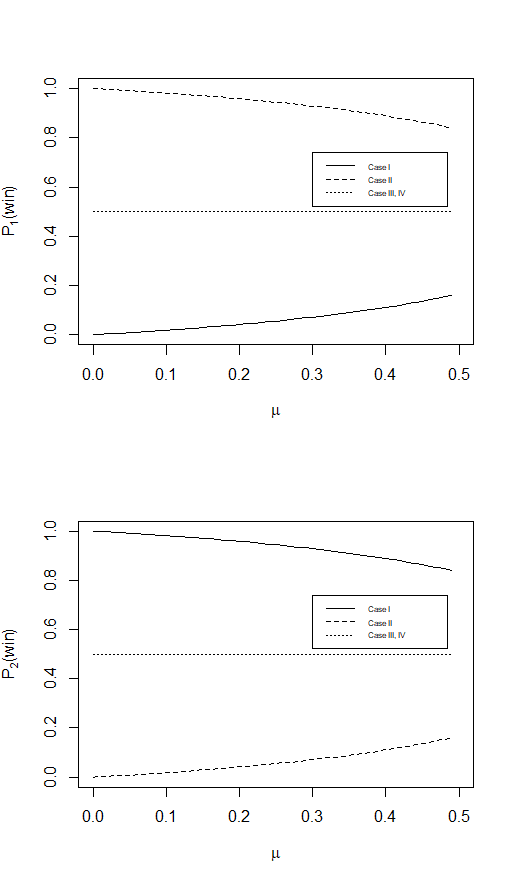
\includegraphics[width=4in]{figures/winprob_with_mu_1_to_2}
\par\end{centering}
\caption{\label{fig:Probability-of-winning}Probability of winning $P_{1}(\text{win})$,
$P_{2}(\text{win})$ for poor and rich participants with varying $\mu$}
\end{figure}


\subsubsection{Intertemporal Choice}

The participants optimise an intertemporally additive utility over
their life-time - which is represented with two time-horizons. The
second-time horizon is set to be one before the end of life when all
wealth accumulated by either participant must disappear. With no accumulations
at the end of life, both rich and poor participants must decide to
spend all their incomes $y_{1}$ or $y_{2}$ (for poor and rich participants
respectively so that $y_{1}<y_{2}$) towards the promotion game. In
the first-stage, however, the participants decide the amount to be
spent towards promotion based upon the utility from wealth they obtain
across the two time-horizons that span their lifetime. For the poor
participant, the total utility to be optimised (assuming EUT) under
the intertemporally additive utility $u(\cdot)$, a winning probability
function $W(x)$ (for expenditure $x$) and a discount-factor $\delta$
is 

\begin{align*}
u(y_{1}-\nu_{1})+\frac{1}{\delta}((1-W(y_{1}))u(y_{1})+W(y_{1})u(y_{2}))
\end{align*}

Similarly, for the rich participant, the total utility to be optimised
(assuming EUT) is 
\begin{align*}
u(y_{2}-\nu_{2})+\frac{1}{\delta}((1-W(y_{2}))u(y_{1})+W(y_{2})u(y_{2}))
\end{align*}

\begin{table}[H]
\begin{centering}
\begin{tabular}{>{\centering}p{0.7in}>{\centering}p{0.7in}>{\raggedright}m{1.5in}|>{\raggedright}m{1.5in}}
 &  & \multicolumn{1}{>{\raggedright}m{1.5in}}{Poor} & participant\tabularnewline
\begin{singlespace}
\end{singlespace}
 & \begin{singlespace}
\end{singlespace}
 & \begin{singlespace}
{\small\textit{withdraws}}
\end{singlespace}
 & \begin{singlespace}
{\small\textit{participates}}
\end{singlespace}
\tabularnewline
\begin{singlespace}
Rich
\end{singlespace}
 & \begin{singlespace}
{\small\textit{withdraws}}
\end{singlespace}
 & \multirow{1}{1.5in}{Case III} & Case II\tabularnewline
\cline{3-4}
\begin{singlespace}
Participant
\end{singlespace}
 & \begin{singlespace}
{\small\textit{participates}}
\end{singlespace}
 & \begin{singlespace}
Case I
\end{singlespace}
 & \begin{singlespace}
Case IV
\end{singlespace}
\tabularnewline
\end{tabular}
\par\end{centering}
\caption{\label{tab:prisoners_dilemma_cases}Cases I,II, III, IV as participant
strategies}
\end{table}

\begin{table}[H]
\begin{raggedright}
{\footnotesize{}%
\begin{tabular*}{1.2in}{@{\extracolsep{\fill}}>{\raggedright}p{0.5in}>{\raggedright}p{0.4in}>{\centering}m{2.5in}|>{\raggedright}m{2.2in}}
 &  & \multicolumn{1}{>{\centering}m{2.5in}}{\begin{onehalfspace}
{\footnotesize Poor}
\end{onehalfspace}
} & \begin{onehalfspace}
{\footnotesize participant}
\end{onehalfspace}
\tabularnewline
 &  & \begin{onehalfspace}
{\footnotesize\textit{withdraws}}
\end{onehalfspace}
 & \begin{onehalfspace}
{\footnotesize\textit{participates}}
\end{onehalfspace}
\tabularnewline
{\footnotesize Rich}\\
{\footnotesize participant} & {\footnotesize\textit{withdraws}} & {\footnotesize
\begin{gather*}
u(y_{2})+\frac{(1-\frac{P}{N})u(y_{2})+\frac{P}{N}u(y_{1})}{\delta}
\end{gather*}
}\\
{\footnotesize
\begin{gather*}
u(y_{1})+\frac{(1-\frac{P}{N})u(y_{2})+\frac{P}{N}u(y_{1})}{\delta}
\end{gather*}
} & {\footnotesize
\begin{gather*}
u(y_{2})+\frac{u(y_{2})p_{2}'+(1-p_{2}')u(y_{1})}{\delta}
\end{gather*}
}\\
{\footnotesize
\begin{gather*}
u(y_{1}-\overline{\nu})+\frac{u(y_{2})p_{1}'+(1-p_{1}')u(y_{1})}{\delta}
\end{gather*}
}\tabularnewline
\cline{2-4}
 & {\footnotesize\textit{participates}} & {\footnotesize
\begin{gather*}
u(y_{2}-\overline{\nu})+\frac{p_{2}u(y_{2})+(1-p_{2})u(y_{1})}{\delta}
\end{gather*}
}\\
{\footnotesize
\begin{gather*}
u(y_{1})+\frac{p_{1}u(y_{2})+(1-p_{1})u(y_{1})}{\delta}
\end{gather*}
} & {\footnotesize
\begin{gather*}
u(y_{2}-\overline{\nu})+\frac{(1-\frac{P}{N})u(y_{2})+\frac{P}{N}u(y_{1})}{\delta}
\end{gather*}
 }\\
{\footnotesize
\begin{gather*}
u(y_{1}-\overline{\nu})+\frac{(1-\frac{P}{N})u(y_{2})+\frac{P}{N}u(y_{1})}{\delta}
\end{gather*}
}\tabularnewline
\end{tabular*}}{\footnotesize\par}
\par\end{raggedright}
\caption{\label{tab:prisoners_dilemma}Utility for poor and rich participants}
\end{table}

\noindent

With above utilities, we now discuss the conditions for whether the
Case I, II, III, IV can become Nash equilibria (see Table \ref{tab:prisoners_dilemma_cases})
or not - and detail the implications for the effect of income differences
on social capital expenditure\footnote{The discussion of the effect of the threshold $\overline{\nu}$ and
the income differences $y_{2}-y_{1}$ on participation (expenditure)
assumes that the exogenous parameter $\mu$ is stable with respect
to short-term changes in threshold investment $\overline{\nu}$ as
well as disposable incomes $y_{1},y_{2}$. }. For ease of notation we define $p_{1},p_{2},p_{1}'$ and $p_{2}'$
as the following:

\begin{gather}
p_{1}\equiv\frac{\mu}{6(1-\mu)}\nonumber \\
p_{2}\equiv1-p_{1}\nonumber \\
p_{1}'\equiv\frac{6-7\mu}{6(1-\mu)}\label{eq:probabilities_2player}\\
p_{2}'\equiv1-p_{1}'\nonumber 
\end{gather}
 

The choices for the poor and rich participants using a general intertemporally
additive function $u(A)$ (for assets $A$) are shown in Table \ref{tab:prisoners_dilemma}.
As we can verify from Figure \ref{fig:Probability-of-winning} that
we have $p_{1}<1/2<p_{2}$ and $p_{1}'>1/2>p_{2}'$ for all values
of $\mu<1/2$.

\begin{gather}
\text{Given }\mu<1/2,\text{we have}\label{eq:probability_inequality}\\
p_{1}<1/2<p_{2}\nonumber \\
p_{1}'>1/2>p_{2}'\nonumber 
\end{gather}
 

Table \ref{tab:prisoners_dilemma} represents the condition when the
budget is non-binding i.e. the poor participant is able to spend $\overline{\nu}$.
i.e. $\overline{\nu}<y_{1}<y_{2}$. When the poor participant faces
a binding constraint i.e. $y_{1}<\overline{\nu}<y_{2}$ , then the
rich participant knows that the best case probability to win for the
poor participant is $\frac{1}{2}$. The rich participant's decision
to participate would depend only on utility from savings and the relative
advantage from gain in probability. This is elaborated in Section
\ref{subsec:Binding-constraint}.

\subsubsection{\label{subsec:Binding-constraint}Binding constraint}

\noindent

Assuming EUT participants, we now consider the simpler case of binding
constraint $y_{1}<\overline{\nu}<y_{2}$. Considering pure strategies
for participation\footnote{With the assumption of a stability in long-term participant behaviour
(which itself is a result of observed probability of success), mixed-strategies
are not relevant in the current set up.}, the rich participant would thus participate only when the utility
from participating would be higher than from not participating i.e.
$u(y_{2}-\overline{\nu})+\frac{p_{2}u(y_{2})+(1-p_{2})u(y_{1})}{\delta}>u(y_{2})+\frac{u(y_{2})+u(y_{1})}{2\delta}$
. This results in the following condition

\begin{align*}
\frac{(p_{2}-1/2)(u(y_{2})-u(y_{1}))}{\delta} & >u(y_{2})-u(y_{2}-\overline{\nu})
\end{align*}

With income differences held constant, an increase in participation
cost $\overline{\nu}$ discourages participation since RHS increases
with $\overline{\nu}$ ($\because u(y_{2}-\overline{\nu})$ is decreasing
in $\overline{\nu}$) and may fail the above condition. Similarly,
with participation cost $\overline{\nu}$ held constant, an increase
in income-difference $y_{2}-y_{1}$ is in the rich participant's interest
whereas a narrowing of income differences reduces incentive for the
participant to participate by possibly failing the above condition.
All else being the same, higher impatience (lower time-discounted
value of money or a higher $\delta$) would also discourage participation.
Therefore, when budget is binding for the poor participant i.e. if
the poor participant cannot participate due to $y_{1}<\overline{\nu}$,
then narrower income differences, higher participation costs and higher
patience for savings (common for both rich and poor participants)
all encourage the rich participant to withdraw from the game. This
also means that wider income differences ($y_{2}-y_{1}$) combined
with lower participation costs ($\overline{\nu}$) may together help
maintain the equilibrium where only the rich participates. Similarly,
wider income differences ( higher $y_{2}-y_{1}$ ) and more patience
for savings (higher $\delta$) would together maintain the incentive
for the rich participant to participate.

\subsubsection{\label{subsec:Non-Binding-constraint}Non-Binding constraint}

\noindent

When budget is non-binding, then participation of the rich participant
is her dominant strategy if the condition is also $u(y_{2})+\frac{u(y_{2})p_{2}'+(1-p_{2}')u(y_{1})}{\delta}<u(y_{2}-\overline{\nu})+\frac{u(y_{2})+u(y_{1})}{2\delta})$
i.e. 

\begin{align*}
\frac{(1/2-p_{2}')(u(y_{2})-u(y_{1}))}{\delta} & >u(y_{2})-u(y_{2}-\overline{\nu})
\end{align*}

The inferences on how $y_{2}-y_{1}$, $\overline{\nu}$ and $\delta$
influence the participation (see Section \ref{subsec:Binding-constraint})
remain the same for the above condition. To discuss the more general
Nash equilibria, consider the conditions for all of the Cases I, II,
III and IV to become a Nash equilibrium. For ease of notation we define
the following for a given $\overline{\nu},y_{1}$ and $y_{2}$

\begin{align*}
U_{1} & \equiv u(y_{1})-u(y_{1}-\overline{\nu})
\end{align*}

\begin{align*}
U_{2} & \equiv u(y_{2})-u(y_{2}-\overline{\nu})
\end{align*}

One could view $U_{1}$ and $U_{2}$ as the immediate gain in wealth
utility from withdrawing. If $u(\cdot)$ represents a diminishing
utility, then it is also necessary for $y_{1}<y_{2}$ that 

\begin{align*}
U_{2} & <U_{1}
\end{align*}

Consider now that conditions for Case I to be a Nash Equilibrium.
If Case I were to be a Nash equilibrium, then for the rich participant's
decision to participate, the poor participant must get more utility
from withdrawing than from participating and for poor participant's
decision to withdraw, the rich must get more utility from participating
than from withdrawing. The following conditions \footnote{$u(y_{1})+\frac{p_{1}u(y_{2})+(1-p_{1})u(y_{1})}{\delta}>u(y_{1}-\overline{\nu})+\frac{\frac{1}{N}u(y_{2})+\frac{1}{N}u(y_{1})}{\delta}\Rightarrow u(y_{1})-u(y_{1}-\overline{\nu})>\frac{(\frac{1}{N}-p_{1})(u(y_{2})-u(y_{1}))}{\delta}$
and $u(y_{2}-\overline{\nu})+\frac{p_{2}u(y_{2})+(1-p_{2})u(y_{1})}{\delta}>u(y_{2})+\frac{\frac{1}{N}u(y_{2})+\frac{1}{N}u(y_{1})}{\delta}\Rightarrow u(y_{2})-u(y_{2}-\overline{\nu})<\frac{(p_{2}-1/N)(u(y_{2})-u(y_{1}))}{\delta}$} must therefore hold simultaneously

\begin{gather}
\frac{(\frac{1}{N}-p_{1})(u(y_{2})-u(y_{1}))}{\delta}<U_{1}\nonumber \\
U_{2}<\frac{(p_{2}-1/N)(u(y_{2})-u(y_{1}))}{\delta}\label{eq:caseI_inequalities}
\end{gather}

Since $p_{2}-\frac{1}{N}\ge\frac{1}{N}-p_{1}$ (strict inequality
follows when the number of poor participants $P$ is higher than that
for rich participants $N-P$ e.g., with $N=3$ and $P=2$), this is
a fairly general condition for the equilibrium. An increase in $U_{1}$
due to higher $\overline{\nu}$ does not change the equilibrium conditions
so long as the corresponding rise $U_{2}$ (due to higher $\overline{\nu}$
) does not affect the second inequality. In other words, a higher
$\overline{\nu}$ favours the equilibrium (Case I) so long as there
is an incentive for the rich to participate. Likewise, a decrease
in $\overline{\nu}$ would be favourable for the equilibrium (Case
I) so long as the poor participants do not also have an incentive
to participate. 

Similar effects can be seen with income differences $y_{2}-y_{1}$
(which increase $u(y_{2})-u(y_{1})$ as well as $\frac{U_{2}}{U_{1}}$)
if we rewrite Equation \ref{eq:caseI_inequalities} as 

\begin{gather*}
\frac{(\frac{1}{N}-p_{1})}{\delta}<\frac{U_{1}}{u(y_{2})-u(y_{1})}\\
\frac{U_{2}}{(u(y_{2})-u(y_{1}))}<\frac{(p_{2}-1/N)}{\delta}
\end{gather*}

Limiting our attention to cases when $\overline{\nu}<y_{1}$, higher
$y_{2}$ for fixed $y_{1}$ decreases $\frac{U_{2}}{u(y_{2})-u(y_{1})}$and
makes it more likely for the rich to participate while it also decreases$\frac{U_{1}}{u(y_{2})-u(y_{1})}$
by raising the stakes enough for the poor to participate (making it
less likely for first inequality to be fulfilled). It is easy to see
that higher impatience $\delta$ encourages both poor and rich to
withdraw. As would be evident, the equilibrium conditions corresponding
to Case II are far more stringent.

If Case II is a Nash Equilibrium, then for rich's decision to withdraw,
the poor participant should get more utility from participating than
from withdrawing and for poor participant's decision to participate,
the rich participant should get more utility from withdrawing than
from participating. This means that the following hold \footnote{$u(y_{1}-\overline{\nu})+\frac{p_{1}'u(y_{2})+(1-p_{1}')u(y_{1})}{\delta}>u(y_{1})+\frac{\frac{1}{N}u(y_{2})+\frac{1}{N}u(y_{1})}{\delta}\Rightarrow u(y_{1})-u(y_{1}-\overline{\nu})<\frac{(p_{1}'-1/N)(u(y_{2})-u(y_{1}))}{\delta}$
and $u(y_{2})+\frac{p_{2}'u(y_{2})+(1-p_{2}')u(y_{1})}{\delta}>u(y_{2}-\overline{\nu})+\frac{\frac{1}{N}u(y_{2})+\frac{1}{N}u(y_{1})}{\delta}\Rightarrow u(y_{2})-u(y_{2}-\overline{\nu})>\frac{(1/N-p_{2}')(u(y_{2})-u(y_{1}))}{\delta}$} simultaneously, 

\begin{gather*}
U_{1}<\frac{(p_{1}'-1/N)(u(y_{2})-u(y_{1}))}{\delta}\\
U_{2}>\frac{(1/N-p_{2}')(u(y_{2})-u(y_{1}))}{\delta}
\end{gather*}

Since $\frac{(p_{1}'-1/N)(u(y_{2})-u(y_{1}))}{\delta}<\frac{(1/N-p_{2}')(u(y_{2})-u(y_{1}))}{\delta}$
, the above cannot be satisfied so long as we have a diminishing utility
which necessitates $U_{2}<U_{1}$. Thus an equilibrium with Case II
which incentivises the poor to participate but not the rich is possible
only with a reference dependent utility with $U_{1}<U_{2}$. With
$U_{1}<U_{2}$, we can write above as 

\begin{gather*}
\frac{U_{1}}{u(y_{2})-u(y_{1})}<\frac{(p_{1}'-1/N)}{\delta}<\frac{(1/N-p_{2}')}{\delta}<\frac{U_{2}}{u(y_{2})-u(y_{1})}
\end{gather*}

Notice that despite a reference-dependent utility, a higher $\overline{\nu}$
or more impatience ($\delta$) may disincentivise the poor from participation
just the same (leading to Case III). Similarly, higher income differences
(an increase in $y_{2}$ for fixed $y_{1}$) could encourage the rich
to participate by decreasing $\frac{U_{2}}{u(y_{2})-u(y_{1})}$ (leading
to Case IV). Even with the reference dependent utility, the equilibrium
with Case II remains a fragile one.

If Case III were to be a Nash-Equilibrium, then for rich participant's
decision to withdraw, poor should get more utility from withdrawing
than from participating and for poor participant's decision to withdraw,
the rich participant should get more from withdrawing than from participating.
The following should thus hold\footnote{$u(y_{1})+\frac{\frac{1}{N}u(y_{2})+\frac{1}{N}u(y_{1})}{\delta}>u(y_{1}-\overline{\nu})+\frac{p_{1}'u(y_{2})+(1-p_{1}')u(y_{1})}{\delta}\Rightarrow u(y_{1})-u(y_{1}-\overline{\nu})>\frac{(p_{1}'-\frac{1}{N})(u(y_{2})-u(y_{1}))}{\delta}$
and $u(y_{2})+\frac{\frac{1}{N}u(y_{2})+\frac{1}{N}u(y_{1})}{\delta}>u(y_{2}-\overline{\nu})+\frac{p_{2}u(y_{2})+(1-p_{2})u(y_{1})}{\delta}\Rightarrow u(y_{2})-u(y_{2}-\overline{\nu})>\frac{(p_{2}-\frac{1}{N})(u(y_{2})-u(y_{1}))}{\delta}$},

\begin{gather*}
U_{1}>\frac{(p_{1}'-\frac{1}{N})(u(y_{2})-u(y_{1}))}{\delta}\\
U_{2}>\frac{(p_{2}-\frac{1}{N})(u(y_{2})-u(y_{1}))}{\delta}
\end{gather*}

Since $p_{1}'-\frac{1}{N}\le p_{2}-\frac{1}{N}$ (strict inequality
when number of poor participants is higher), we have $\frac{(p_{1}'-\frac{1}{N})(u(y_{2})-u(y_{1}))}{\delta}<\frac{(p_{2}-\frac{1}{N})(u(y_{2})-u(y_{1}))}{\delta}$
and $U_{2}<U_{1}$ . A higher $\overline{\nu}$ pushes both $U_{2}$
and $U_{1}$ further away from participation but a fall in $\overline{\nu}$,
incentivises the rich participant to participate (leading to Case
I). 

\begin{gather*}
\frac{U_{1}}{u(y_{2})-u(y_{1})}>\frac{(p_{1}'-\frac{1}{N})}{\delta}\\
\frac{U_{2}}{u(y_{2})-u(y_{1})}>\frac{(p_{2}-\frac{1}{N})}{\delta}
\end{gather*}

Higher income differences i.e. higher $y_{2}$ for fixed $y_{1}$
also decrease $\frac{U_{2}}{u(y_{2})-u(y_{1})}$ and incentivise the
rich participant to participate (leading to an equilibrium with Case
I). Conversely, if the game is not lucrative for the rich it would
automatically be infeasible for the poor i.e. if rich withdraws then
poor automatically withdraws. If there is any net utility from playing
the game, however, Case IV is the likely equilibrium.

If Case IV were to be a Nash Equilibrium, then for rich's decision
to participate, the poor participant should get more from participating
than from withdrawing and for poor's decision to participate, the
rich participant should get more from participating than from withdrawing.
Therefore, the following\footnote{$u(y_{1}-\overline{\nu})+\frac{\frac{1}{N}u(y_{2})+\frac{1}{N}u(y_{1})}{\delta}>u(y_{1})+\frac{p_{1}u(y_{2})+(1-p_{1})u(y_{1})}{\delta}\Rightarrow u(y_{1})-u(y_{1}-\overline{\nu})<\frac{(\frac{1}{N}-p_{1})(u(y_{2})-u(y_{1}))}{\delta}$
and $u(y_{2}-\overline{\nu})+\frac{\frac{1}{N}u(y_{2})+\frac{1}{N}u(y_{1})}{\delta}>u(y_{2})+\frac{p_{2}'u(y_{2})+(1-p_{2}')u(y_{1})}{\delta}\Rightarrow u(y_{2})-u(y_{2}-\overline{\nu})<\frac{(\frac{1}{N}-p_{2}')(u(y_{2})-u(y_{1}))}{\delta}$} must hold

\begin{gather*}
U_{1}<\frac{(\frac{1}{N}-p_{1})(u(y_{2})-u(y_{1}))}{\delta}\\
U_{2}<\frac{(\frac{1}{N}-p_{2}')(u(y_{2})-u(y_{1}))}{\delta}
\end{gather*}

With $\frac{(\frac{1}{N}-p_{2}')(u(y_{2})-u(y_{1}))}{\delta}<\frac{(\frac{1}{N}-p_{1})(u(y_{2})-u(y_{1}))}{\delta}$
and $U_{2}<U_{1}$ , this equilibrium rests upon the incentive for
the poor participant to participate. So long as the poorer participant
finds the competition worthwhile, the rich would also participate. 

The above results outline how participation costs influence the investments
towards status. For very low $\overline{\nu}$, rich and poor would
both participate and for very high $\overline{\nu}$, both would withdraw.
For everything in between, the only equilibrium may be the one where
only the rich participate. A reference-based utility may permit an
equilibrium but at the likely cost of segregation of income classes.

\section{\label{sec:Conclusion}Conclusion}

\noindent 

The paper examines how inequality can shape social capital investments---particularly
education---when status is endogenised as both a determinant and
an outcome of mobility. By considering the signaling value of education
modeled as small-scale tournaments combining innate ability and social
capital, the analysis links income differences, participation costs,
and reference-dependent utility to long-term patterns of educational
expenditure.

Three principal findings emerge. First, inequality can initially stimulate
social capital investments, but excessive inequality makes status
competitions unsustainable unless participation costs adjust accordingly.
Second, participation costs are crucial: when they remain high, only
the rich participate in status-related investments such as education,
while lower costs allow both rich and poor to compete. Status competitions
imply that a rise in inequality increases social capital expenditures
when participation costs are held constant. The presence of signaling
thus necessitates that participation costs rise to sustain limits
to mobility. Status consideration, participation costs and inequality
remain intricately linked so long as status competitions exist in
a society. Reducing income-differences without lowering of participation
costs in status competitions may have an effect of supporting status-related
competitions under long-established inequalities. Third, under diminishing
utility of wealth, the model admits only two stable long-run equilibria---either
universal participation in status competitions or participation limited
to the rich. These outcomes quantitatively formalize earlier qualitative
arguments about the social limits to growth and mobility \cite{HirschSocialLimits,GalbraithAffluent,GalbraithBeyondContentment1994}.

The inclusion of reference-dependent utility further highlights how
perceived contentment can sustain segregation of competitions even
under large income gaps---consistent with empirical evidence on meritocratic
beliefs amid inequality \cite{MijsMeritocracy2020}. Together, these
results reveal a dynamic interplay between inequality, participation
costs, and status incentives. For education policy, they suggest that
mobility cannot be expanded merely by widening access or increasing
expenditure; the signaling role of education and the costs of participation
must also be managed to prevent inequality from reproducing itself
through status-driven competition.

\bibliographystyle{apacite}
\bibliography{status_consumption} 

\begin{appendices}
\section{Convolution of Uniform Random Variables} \label{sec:appendix_theorertical_1}

The distribution of a convex combination $w=\mu r+(1-\mu)s$ of two
random variables $r,s$ - which are distributed according to densities
$f_{R}(r)$ and $f_{S}(s)$ - can be derived using the convolution
of two derived variables $x=\mu r$ and $y=(1-\mu)s$. If $r$ and
$s$ are uniformly distributed variables ranging from 0 to 1, then
$x$ ranges from 0 to $\mu$ and $y$ ranges from $0$ to $(1-\mu)$.
The CDF for $F_{X}(x)$ and $F_{Y}(y)$ are simply $F_{X}(x)=\frac{x}{\mu}$
, $F_{Y}(y)=\frac{y}{1-\mu}$ (respectively). Therefore, the densities
for $x$ and $y$ are $f_{X}(x)=\frac{1}{\mu}$ and $f_{Y}(y)=\frac{1}{1-\mu}$.
The density of $w$ is simple $f(w)=\int_{-\infty}^{\infty}f_{Y}(w-x)f_{X}(x)dx$.
Since , $f_{X}(x)$ is $1/\mu$ only between $0$ and $\mu$. We have
the following integral to evaluate for the convolution

\begin{align*}
f(w) & =\frac{1}{\mu}\int_{0}^{\mu}f_{Y}(w-x)dx
\end{align*}

Since $f_{Y}(y)$ is 1 only between 0 and $1-\mu$, we have the condition
$0<w-x<1-\mu\Rightarrow w-(1-\mu)<x<w$. Further, $x$ is distributed
only between 0 and $\mu$. As shown in Figure \ref{fig:convex_combo},
the integral would evaluate to the following\footnote{Notice that as a convex combination, $w$ is distributed only between
0 and 1.} under the assumption $\mu<\frac{1}{2}$.

\begin{align*}
f(w)=\frac{1}{\mu}\int_{0}^{\mu}f_{Y}(w-x)dx & =\begin{cases}
\frac{1}{\mu}\int_{0}^{w}\frac{1}{1-\mu}dx & 0<w<\mu\\
\frac{1}{\mu}\int_{0}^{\mu}\frac{1}{1-\mu}dx & \mu<w<1-\mu\\
\frac{1}{\mu}\int_{w-(1-\mu)}^{\mu}\frac{1}{1-\mu}dx & 1-\mu<w<1\\
0 & \text{otherwise}
\end{cases}
\end{align*}

This can be simplified as 

\begin{align*}
f(w) & =\begin{cases}
\frac{w}{\mu(1-\mu)} & 0<w<\mu\\
\frac{1}{1-\mu} & \mu<w<1-\mu\\
\frac{1-w}{\mu(1-\mu)} & 1-\mu<w<1\\
0 & \text{otherwise}
\end{cases}
\end{align*}

Figure \ref{fig:convex_combo_plot} shows this trapezoidal density
with $\mu$ set to $\frac{1}{5}$. The CDF $F_{X}(x)$ can be evaluated
by integrating the above density as $P(X<x)=\int_{-\infty}^{x}f(t)dt$. 

\begin{align*}
F_{X}(x) & =\begin{cases}
\frac{x^{2}}{2\mu(1-\mu)} & 0<x<\mu\\
\frac{\mu}{2(1-\mu)}+\frac{x-\mu}{1-\mu} & \mu<x<1-\mu\\
\frac{\mu^{2}}{2\mu(1-\mu)}+\frac{2\mu(1-2\mu)}{2\mu(1-\mu)}+\frac{\mu^{2}-x^{2}+2x-1}{2\mu(1-\mu)} & 1-\mu<x<1\\
0 & \text{otherwise}
\end{cases}
\end{align*}

Simplifying above, we have

\begin{align*}
F_{X}(x) & =\begin{cases}
\frac{x^{2}}{2\mu(1-\mu)} & 0<x<\mu\\
\frac{x-\mu/2}{1-\mu} & \mu<x<1-\mu\\
1-\frac{(x-1)^{2}}{2\mu(1-\mu)} & 1-\mu<x<1\\
0 & \text{otherwise}
\end{cases}
\end{align*}

\begin{figure}[H]
\begin{centering}
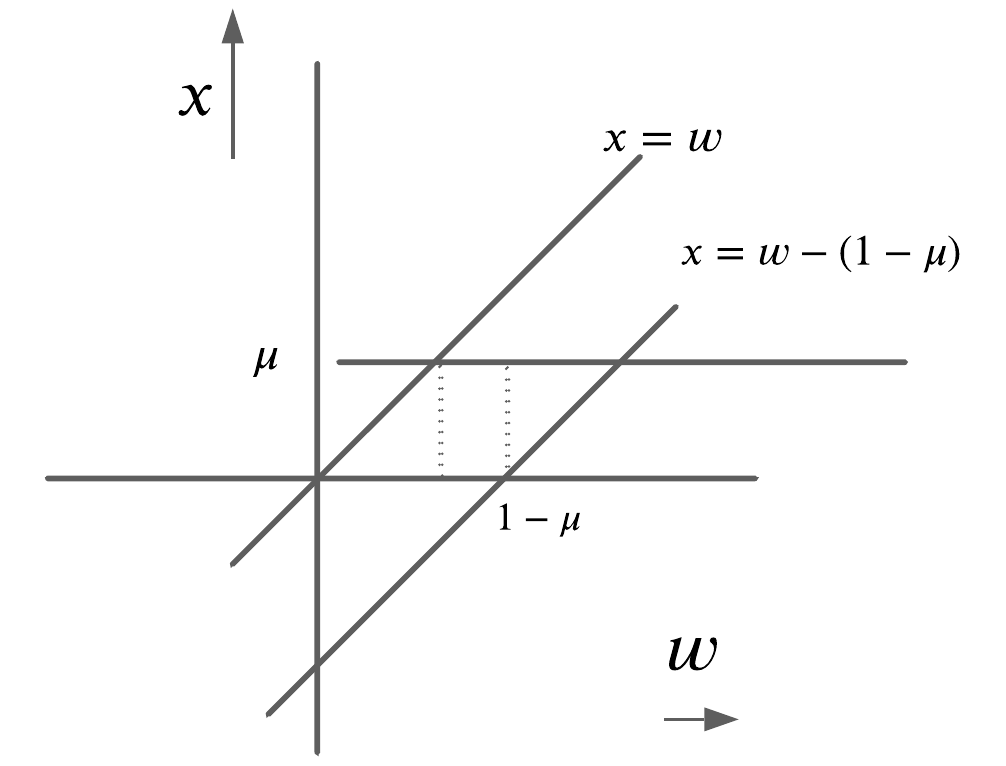
\includegraphics[width=4in]{figures/combined_density}
\par\end{centering}
\caption{\label{fig:convex_combo}Ranges of $w$ and $w-x$ for convolution
of two scaled random variables}
\end{figure}

\begin{figure}[H]
\begin{centering}
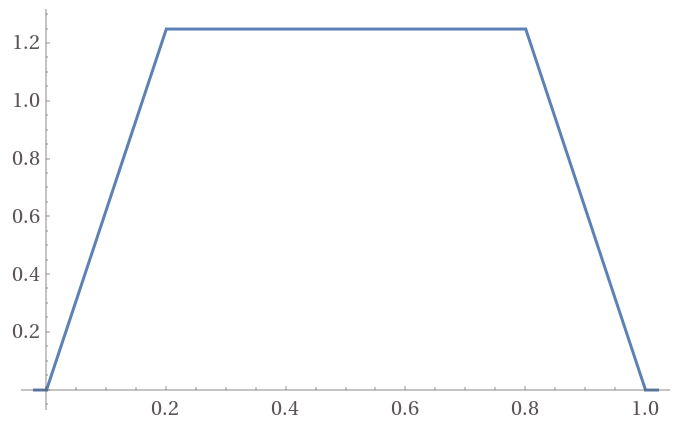
\includegraphics[width=4in]{figures/combined_density_plot}
\par\end{centering}
\caption{\label{fig:convex_combo_plot}Combined density of $w$ as the convex
combination of two random variables with $\mu=\frac{1}{5}$}
\end{figure}

\newpage
\section{$P(\text{win}|r,s)$} \label{sec:appendix_theorertical_2} 

To calculate $\int_{s=0}^{s=1}\int_{r=0}^{r=1}P(\text{win}|r,s)drds$
over the variable $x$ (where $0<r<1$ and $0<s<1$), we evaluate
the sum of three parts split by the boundaries of the piecewise function.
The three parts are shown in Figure \ref{fig:integral_boundaries}.
If $x=\mu r+(1-\mu)s$ and $F(x)$ is of the following piece-wise
form

\begin{align*}
F(x) & =\begin{cases}
A & 0<x<\mu\\
B & \mu<x<1-\mu\\
C & 1-\mu<x<1\\
0 & \text{otherwise}
\end{cases}
\end{align*}

Then the integral $\int_{s=0}^{s=1}\int_{r=0}^{r=1}F(x)drds$ can
be written as

\begin{align*}
\int_{s=0}^{s=1}\int_{r=0}^{r=1}F(x)dsdr & =\int_{r=0}^{r=1}{\int_{s=0}^{s=\frac{\mu(1-r)}{1-\mu}}A\ dsdr}+\int_{r=0}^{r=1}{\int_{s=\frac{\mu(1-r)}{1-\mu}}^{s=1-\frac{\mu r}{1-\mu}}B\ dsdr}+\int_{r=0}^{r=1}{\int_{s=1-\frac{\mu r}{1-\mu}}^{s=1}C\ dsdr}
\end{align*}

\begin{figure}[h]
\begin{centering}
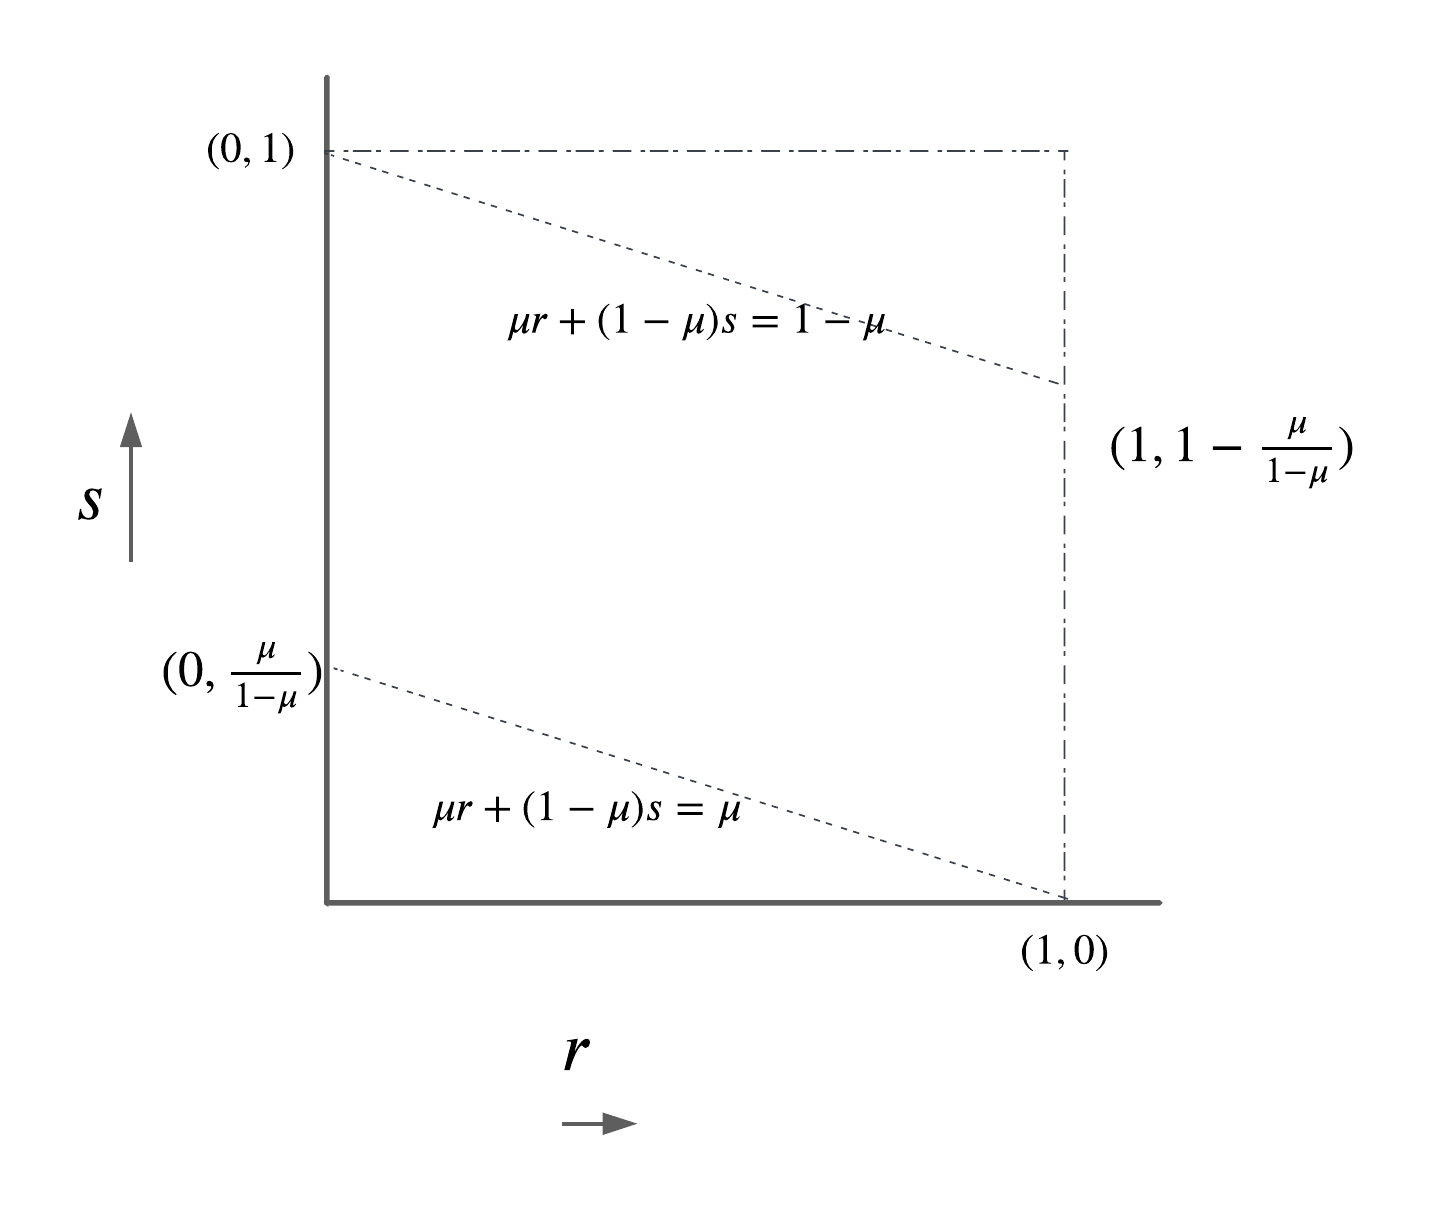
\includegraphics[width=4in]{figures/integral_calculation}
\par\end{centering}
\caption{\label{fig:integral_boundaries}Integration over $r,s$ split by boundaries
$\mu r+(1-\mu)s=\mu$ and $\mu r+(1-\mu)s=1-\mu$}
\end{figure}

\end{appendices}
\end{document}
